\documentclass[11pt,a4j,notitlepage]{jsarticle}
\usepackage{TUSGradThesis}

\usepackage[dvipdfmx]{graphicx}
\usepackage[dvipdfmx]{color}
\usepackage{amsmath,amssymb}
\usepackage{setspace}
\usepackage{fancyhdr}
\usepackage{amsmath}
\usepackage{bm}
\usepackage{here}
\usepackage{multirow}
\usepackage{ascmac}
\usepackage[dvipdfmx]{color}
\usepackage{subfigure}
\usepackage{cases}
\usepackage{setspace}
\usepackage{subfiles}
\usepackage{algorithm}
\usepackage{algorithmic}
\usepackage{afterpage}
\usepackage{comment}

\makeatletter
    \renewcommand{\theequation}{%
    \thesection.\arabic{equation}}
    \@addtoreset{equation}{section}
    \def\thefigure{\thesection.\arabic{figure}}
    \@addtoreset{figure}{section}
    \renewcommand{\thetable}{%
    \thesection.\arabic{table}}
    \@addtoreset{table}{section}
\makeatother

\renewcommand\bibname{参考文献}
\newcommand{\Figref}[1]{図~\ref{#1}}
\newcommand{\Eqref}[1]{式~(\ref{#1})}
\newcommand{\Tabref}[1]{表~\ref{#1}}

\newcommand{\mymax}{\mathop{\rm max}\limits}

\makeatletter
\renewcommand{\l@figure}{\@dottedtocline{1}{1.5em}{3.2em}}
\makeatother

\makeatletter
\renewcommand{\l@table}{\@dottedtocline{1}{1.5em}{3.2em}}
\makeatother

\makeatletter
\newcommand{\subsubsubsection}{\@startsection{paragraph}{4}{\z@}%
  {1.0\Cvs \@plus.5\Cdp \@minus.2\Cdp}%
  {.1\Cvs \@plus.3\Cdp}%
  {\reset@font\normalsize\bfseries}
}
\makeatother
\setcounter{secnumdepth}{4}

\setstretch{1.0}
\setcounter{tocdepth}{2}
%\setcounter{secnumdepth}{3}

% 表紙情報
\発表年度{2021} % 全角で書くこと
\著者情報{4618023}{北田 来人}
\指導教員{藤井 孝藏 1教授,松尾 裕一 教授}{立川 智章 准教授, 浅田 健吾 助教}
\論文題目{多目的進化計算における}{設計変数の削減方法に関する研究}
{Research of reducing decision variables}{in Multi Objective Evolutionary Algorithm}
\pagestyle{empty}
% 要旨
%\要旨{}
\begin{document}
% 表紙の出力
\begin{center}
\LARGE{多目的進化計算における設計変数の削減方法に関する研究}
\end{center}
\begin{flushright}
北田来人 (藤井 孝藏 教授,立川 智章 准教授, 松尾 裕一 教授, 浅田 健吾 助教)
\end{flushright}
\vspace{-1.75zh}
\section {はじめに}
\vspace{-1.0zh}
進化計算は数値最適化,組合せ最適化,制約最適化など様々な場面で利用されている.それに伴い実問題においても進化計算が利用され,限られた計算回数で,設計変数の数が莫大な多目的最適化(Large Scale Global Optimization)問題を解くことは強く求められている.例えば,車体設計情報抽出に適した多目的可視化に関する研究[多田]では車体の部品を設計変数として用いる際に,200以上の設計変数が使用された.また,空気力学の形状最適化問題での設計変数は何千もあると記載\cite{Tada}されている.多目的進化計算には計算コストの増加,最適化の遅延が起こる代表的な3つの課題が存在する.1つ目の課題として今でも幅広く利用,拡張されるNSGA-IIなどのパレート支配に基づく多目的進化計算手法を困難にすること.これは目的関数の数が増大することで,解同士が支配関係を有することが難しくなるためである(例えば目的関数の数が20を超え始めると,1000個の解を用意してもパレート最適解がほぼ存在しなくなる\cite{Sato1})
\begin{comment}
  パレート支配は,解集団内の相対比較によって解の優劣が決まるところなどさまざまな問題に対してして,非劣解集合を獲得できる部分に利点がある.そのため
\end{comment}
2つ目の課題として多数の制約条件を部分的にしか満足できない場合や,厳しい制約条件を満足できない場合など,制約条件が原因で最適化を困難にすること.3つ目の課題として設計変数の数が膨大になることで,最適化を困難にすること.図1.1は横軸を関数評価回数NFE,縦軸を多目的最適化の評価指標であるパレートフロントのIGD(値が小さいほど収束性と多様性に優れている最適化問題の指標)の推移図である.計算条件は設計変数の数以外,等しくしており設計変数の数を40,200,1000の場合に分けている.図1.1において設計変数の数が多いほど最適化が進みにくくなっているのがわかる.
\begin{figure}[htbp]
\begin{center}
  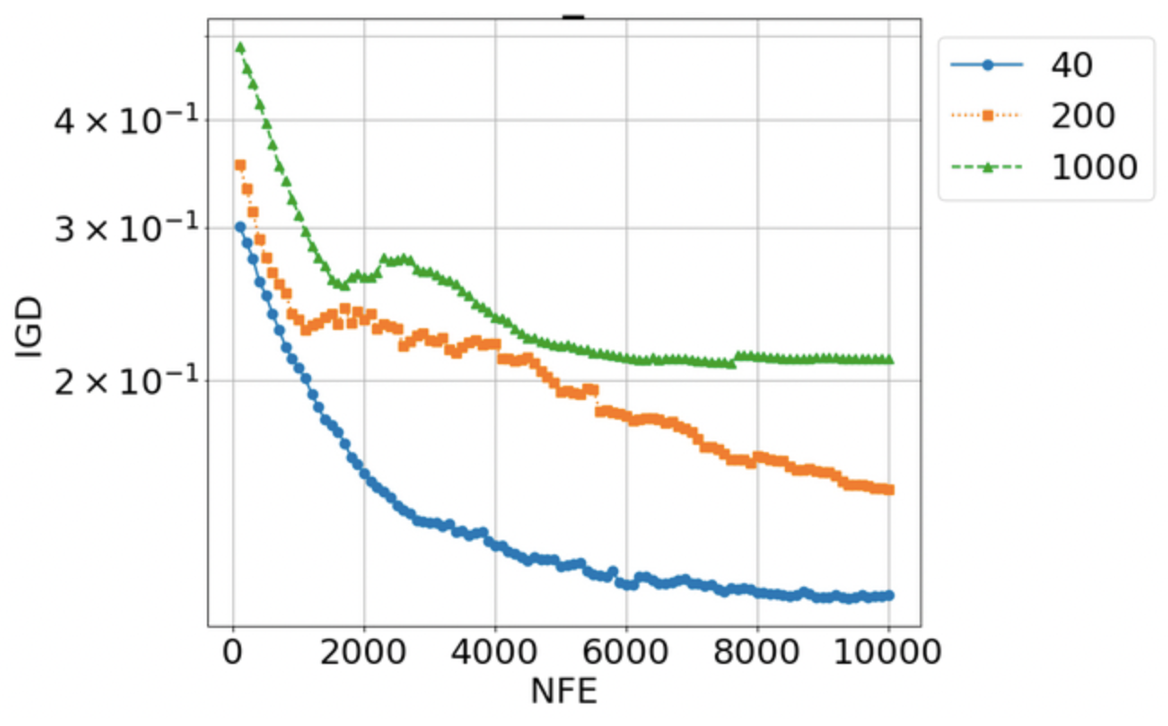
\includegraphics[width=0.5\linewidth]{fig1.png}
             \setlength{\abovecaptionskip}{0mm}
  \setlength{\belowcaptionskip}{0mm}
    \caption{設計変数の違いによる評価値の推移図}
\label{fig:nsgaiii}
\end{center}
\end{figure}
\vspace{-1.5zh}
以上の課題に対し,1つ目の課題に関しては目的関数の削減をするアプローチ\cite{Deb1}やパレート支配の概念を拡張して解集団をより細かいところまでみて優劣付けするアプローチ\cite{HSato}などのさまざまな研究が行われている,2つ目の課題に関しても例えば,第一段階で全ての制約条件を満たす解を差分進化で抽出し,第二段階でその抽出した解から制約条件をより多く満たす上位$x\%$(xはユーザが決める基準値)の解を局所探索アルゴリズムで見つける\cite{Yo}このような2段階探索などの工夫を行い多数目的かつ強制約問題の最適化に対応でき始めている.しかし3つ目の課題,設計変数の数が膨大な場合においては未だ不十分であり,最適化手法に改善の余地がある.ゆえに本研究ではLSGO問題に対して,効果的な方法を提案することを目的とする.
\vspace{-1.5zh}
\section{主成分分析を用いた進化計算手法}
\vspace{-1.5zh}
\subsection{主成分分析(PCA)について}
\vspace{-1.0zh}
主成分分析とは
%元のデータ(データは定量化できない質的変数ではなく量的変数である必要がある)から新しい変数を作ることまた,情報を減らさずに次元を減らす方法である.
元情報n次元の量的変数$x=(x_1,x_2,\cdots ,x_n)$が存在する場合,その係数を掛け合わせて,新たな$x$の特徴を表した値 $y$(これを主成分という)を求めること,またその主成分を新たな変数として$X$の次元を減らす操作のことである.主成分$y$は$x$の線型結合和で次のように表すことができる.
\begin{eqnarray}
  y&=&w_1x_1+w_2x_2+\cdots+w_px_p
\end{eqnarray}
$w=(w_1,w_2,\cdots ,w_n)$を求める際には$x$に関する固有方程式を解く必要がある.
\vspace{-1.5zh}
\subsection{進化計算における主成分分析を用いた設計変数の次元削減の適用}
\vspace{-1.0zh}
本研究では進化計算の個体を生成する部分に工夫を施したものとなっている.新たな個体を生成する際に解$X$を主成分分析を用いてより次元の小さい$X^{\prime}$に変換して交叉を行う.
新たに提案する手法についての流れを以下に示す.また解の設計変数の数を$n$とする.
\vspace{-1.5zh}
\begin{enumerate}
  \item 最初に乱数で個体群を生成する,ここで良い解を生成できれば最適化がよりよく働く
  \item 個体群が環境に適しているかどうかの評価をする
  \item 2.で評価した個体群から必要な数の個体を選択し,親個体群$P$を生成する
  \item 累積非劣解と親個体群に対して,主成分分析を行い、寄与率の合計が$0.95$を超えるまでの固有ベクトルを行列$W$とする.付随して $W$の逆行列$W^{\prime}$を求める.
  \item まず、親個体に$W$を用いて主成分へと変換し次元削減を行い$P^{\prime}$を生成する.その後$P^{\prime}$に交叉を行い新たな個体を生成、生成した個体を$W^{\prime}$で元の次元に戻し個体$Q$を生成.個体$Q$に突然変異を行い、子個体を生成する
  \item 生成した子個体群に対して環境に適しているかどうかの評価をする
  \item 計算は事前に与えられた条件(世代数や関数評価回数)を満たすと終了する.満たしていない場合,評価に応じて選択・淘汰を行う.選ばれた個体は次世代の親個体となり,4へ戻り同様の流れを繰り返すことによって環境に適した個体に進化していく.
\end{enumerate}
\vspace{-1.5zh}
\section{結果と考察}
\vspace{-1.0zh}

\section{終わり}
\vspace{-1.0zh}
SBXを-3~3までにしているが研究を要する

\vspace{-1.0zh}
\begin{thebibliography}{99}
  {\fontsize{10pt}{10pt}\selectfont
\bibitem{Tada}多田 春樹,藤井 孝藏,立川 智章,."車体設計情報抽出に適した多目的可視化に関する研究"
\bibitem{Sato1}佐藤 寛之,石渕 久生."進化型多数目的最適化の現状と課題"

\bibitem{Deb1}K. Deb and K. Saxena." “Searching for Paretooptimal solutions through dimensionality reduction for
certain large-dimensional multi-objective optimization
problems,” In Proeedings of 2006 IEEE Congress on
Evolutionary Computation (CEC 2006), pp. 3353–
3360, 2006."
\bibitem{HSato}H. Sato, H. Aguirre and K. Tanaka, “Controlling
dominance area of solutions and its impact on the performance of MOEAs,” In Proceedings of 2007 Evo
\bibitem{Yo}余 俊, 高木 英行,
“強制約条件付き最適化問題の2段階探索”
\bibitem{Do}鐘 睿,高木 英行."大規模最適化問題へのスパースモデリング導入"
\bibitem{Chai}Chai T, Jin Y, Sendhoff B,"Evolutionary complex
engineering optimization" Opportunities and challenges. IEEE Computational Intelligence Magazine
2013, 8(3):12-15.
}
\end{thebibliography}

\end{document}
